% !TeX spellcheck = hu_HU
% !TeX encoding = UTF-8

% TODO: struktúra meghatározása
\chapter{Virtualizációs környezet létrehozása}
\label{chap:testenv}

\section{Kialakítani kívánt környezet meghatározása}
Dolgozatomban egy kisebb léptékű, de a fontosabb elvek ismertetését kellő mértékben lehetővé tevő tesztkörnyezetet fogok kialakítani és részletesen bemutatni. A tesztkörnyezetben egy fizikai gépen (virtual host) fogok virtuális gépeket kialakítani a \acrshort{kvm} \gls{hypervisor} és a \gls{libvirt} virtualizációs \acrshort{api} segítségével. Ezen környezet célja, hogy betekintést engedjen a nagyvállalati környezetekben alkalmazott virtualizációs rendszerek kialakításának fontosabb lépéseibe.

A \acrshort{kvm}-re és a \gls{libvirt}-re azért esett a választásom, mert ezek modern technológiáknak tekinthetőek, az elmúlt 20 évben jöttek létre, és a mai napig aktívan fejlesztik őket. A \acrshort{kvm} a Linux kernel része, így a támogatottsága egyedülálló, és lényegében minden Linux disztribúción használható. Emellett több nagy szoftvergyártó és felhőszolgáltató (pl. Google, Red Hat) is a \acrshort{kvm}-re építi a saját infrastruktúráját, így a technológia jövője is biztosnak tekinthető~\cite{RedHatVirtKVM}~\cite{GoogleCloudKVM}. A \gls{libvirt} a virtuális gépek könnyű kezelhetőségében segít, mivel az \acrshort{api}-t több fontos virtualizációt kezelő szoftver (pl. virt-manager, virsh, virt-viewer) is implementálja, így egyaránt biztosított a \acrshort{vm}-ek grafikus és a konzolos felületen való kezelése is.
Ezek mellett a \gls{libvirt} számos további kedvező lehetőséget biztosít. Lehetőség van például a virtuális gépek által használt háttértár-partíciók méretének online növelésére, \acrshort{vm}-leíró XML-ek generálására, melyek megkönnyítik a virtuális gépek létrehozását, valamint a gépek másik hosztgépre történő áthelyezésében is könnyebbséget jelentenek.

\section{Fizikai gép ismertetése}

\section{Operációs rendszer}
Értekezésemben nagy szerepe lesz a választott operációs rendszereknek, hiszen ezek fognak a virtualizációs rendszer alapjául szolgálni, valamint képesnek kell lennünk a gépek távoli menedzsmentjére is, így mindenképpen olyan megoldásra van szükség, amely jól támogatott a választott infrastruktúramenedzsment eszköz által. Fontos szempont volt továbbá, hogy a tesztkörnyezet a lehetőségekhez mérten jól reprezentálja a nagyvállalati környezetben használatos rendszereket, így sok olyan OS-verzió kikerült a lehetőségek közül, amelyek ugyan népszerűek például asztali megoldásként, de egyes nagyvállalati szoftverek (legyen az adatbázismotor, vagy bizonyos eszközvezérlők, driverek) hivatalosan nem támogatottak rajtuk. Emiatt az operációs rendszerek kiválasztása során körültekintően jártam el, több Linux-disztribúció is szóba került, az ezekről született konklúziót itt foglalom össze néhány mondatban.

\subsection{OS-kiválasztás folyamata}
Ahogy \aref{sect:os}. alfejezetben is kitértem rá, a nagyvállalatok elsősorban a Red Hat és a SUSE Linux-disztribúciók közül választanak, hiszen ezeknek a velük együtt járó támogatás és a szoftvercsomagok széleskörű támogatottsága miatt kényelmesebb és hatékonyabb az üzemeltetésük, valamint biztonsági szempontból is kedvezőbbek (például gyorsabban kapnak meg bizonyos frissítéseket, patcheket). Szintén jobban támogatottak ezeken a rendszereken a különböző felhasználásspecifikus modulok, például \acrfull{ha}, live patching (támogatás pl. kritikus kernel biztonsági javítások telepítése a számítógép újraindítása nélkül) és real time computing (valós idejű, nagy időbeli pontosságot igénylő alkalmazások futtatására alkalmas környezet).

A fent ismertetett szélesebb körű támogatottság miatt a tesztkörnyezethez használni kívánt operációs rendszerek köre a Red Hat-re és a SUSE Linuxra korlátozódott. A végső döntésben végül az alábbi szempontok segítettek:
\begin{itemize}
	\item a tesztkörnyezetet szerettem volna egy ökoszisztémán belül tudni mind a virtuális gépeket futtató, mind pedig az azokon futó \acrshort{os}-ek esetében,
	\item könnyebb konfigurálhatóság: mivel több gépet kellett telepíteni, így fontos szerepe volt annak, hogy egy-egy operációs rendszer telepítése milyen bonyolultságú,
	\item a környezetet a költségek minimalizálása mellett szerettem volna létrehozni, így lényeges szempont volt, hogy az adott rendszerhez ne kelljen előfizetést vásárolni, mégis a lehető legközelebb álljon a kereskedelmi forgalomban kapható termékekhez.
\end{itemize}

Mindezek figyelembevételével és korábbi tapasztalataim alapján a SUSE termékcsaládja mellett döntöttem. A támogatással rendelkező, előfizetéses modellt használó nagyvállalati változat mellett szabadon beszerezhető openSUSE operációsrendszer-család megfelelt a tesztkörnyezettel szemben támasztott elvárásaimnak. A rendszer telepítését és a későbbi konfigurációt a YaST keretrendszer segíti, mely számos moduljával (pl. particionálás, hálózati és tűzfalbeállítások) nagyban hozzájárul a gépek könnyebb beállításához, kezeléséhez. A YaST -- mivel szervereken való használatra tervezték, melyek gyakran nem rendelkeznek grafikus felülettel -- \aref{fig:yast-partitioner} ábrán látható megjelenés mellet egy konzolos, GUI-szerű (GUI-like) felülettel is rendelkezik, így a konfiguráció kényelmesen elvégezhető konzolos hozzáférés, például \acrshort{ssh} használata esetén is.

% TODO: yast kép olvashatóság ellenőrzése
\begin{figure}[!ht]
	\centering
	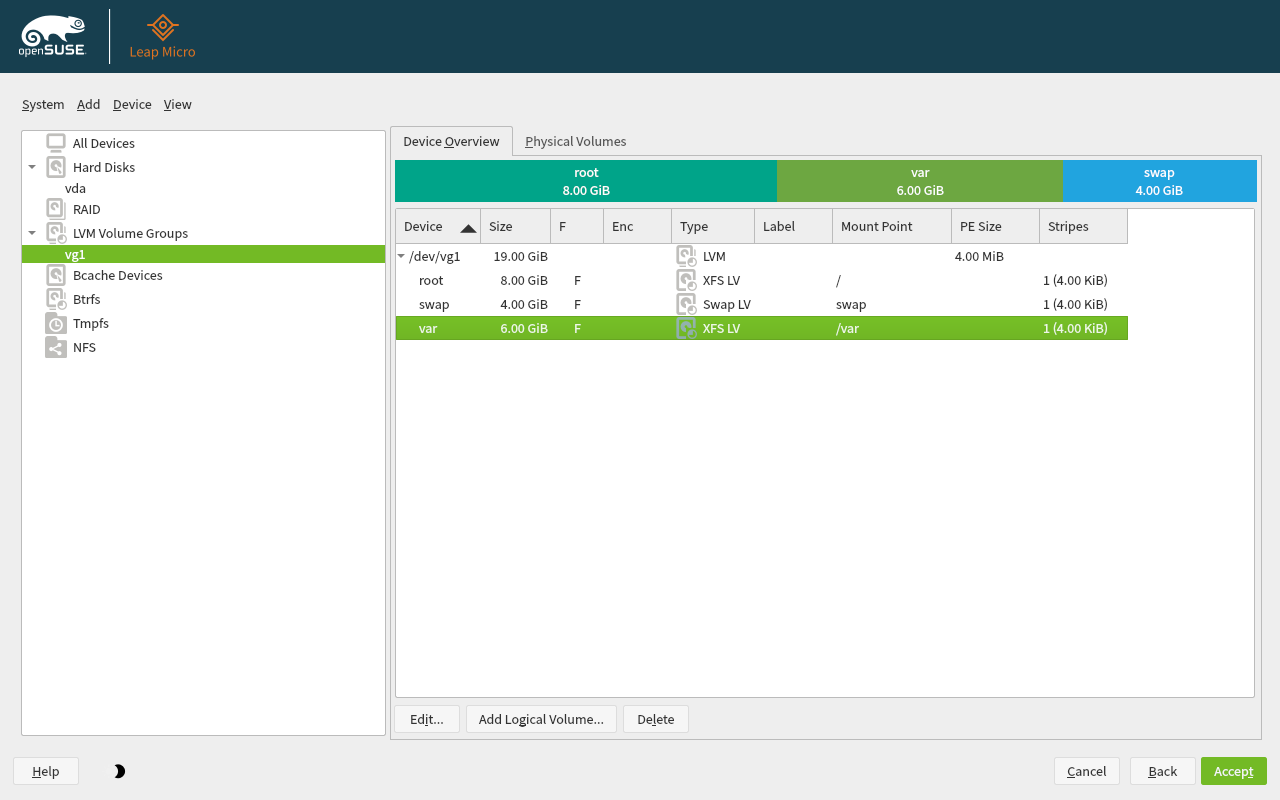
\includegraphics[width=15cm]{figures/yast-partitioner.png}
	\caption{\acrshort{lvm}-kötetek létrehozása openSUSE Leap Micro telepítése során grafikus YaST telepítő segítségével.}
	\label{fig:yast-partitioner}
\end{figure}

Az openSUSE-projekt több operációs rendszert is fejleszt\footnote{\url{https://get.opensuse.org/}}, ezek közül én a tesztkörnyezetben kettőt használtam, melyeket a következő alfejezetekben ismertetek.

\subsubsection{openSUSE Leap}
A Leap egy hagyományos értelemben vett szerver operációs rendszer. Gyakran kap biztonsági frissítéseket, új verziói pedig körülbelül évente jelennek meg. Alapjául a \acrlong{sle} szolgál, melynek előnye, hogy a két rendszer csomagjai binárisan kompatibilisek egymással, azaz egy \acrshort{sle}-rendszerre készített csomag garantáltan használható openSUSE Leap-en is, és fordítva~\cite{openSUSELeap15SP3intro}~\cite{SLE15SP3intro}. Utóbbi előnye, hogy így számos, a közösség (akár a hivatalos openSUSE projekt, akár a felhasználók) által készített csomagot használhatunk a \acrshort{sle}-alapú rendszerünkön is, bár ehhez nem kapunk hivatalos támogatást.

A nagyvállalati rendszerből való leszármazás másik nagy előnye, ami fontos volt számomra a kiválasztási folyamat során, hogy így gyakorlatilag a \acrlong{sle} egy ingyenes verzióját használhatom, mely lényegében teljesen megegyezik a vállalati környezetben használt megoldással, és előfizetés nélkül is kap frissítéseket, így folyamatosan naprakészen tartható. A biztonsági javításokat illetően fontos megjegyezni, hogy a Leap rendelkezik egy olyan csomagforrással (repository) is, mely a \acrlong{sle}-ban is elérhető frissítéseket tartalmazza, így az ott hozzáférhető fontos javításokat is telepíthetjük a Leap-et futtató rendszereinkre~\cite{openSUSELeapSLERepo}.

\subsubsection{openSUSE MicroOS}
A MicroOS egy újfajta megközelítést használó, modern operációs rendszer, mely elsősorban konténerizált alkalmazások futtatásához készült. \Az{\acrshort{os}} előnye, hogy az alap installáció csak egy minimális szoftvercsomagot tartalmaz, így az erőforrásigénye elenyésző. A MicroOS egy írásvédett (read-only) BTRFS gyökérkönyvtárral rendelkezik, melynek előnye, hogy magas szintű támogatást nyújt fájlrendszer-pillanatképek (filesystem snapshots) kezelésére.
Erre a technológiára épít a MicroOS filozófiája: atomi frissítéseket támogat, ami azt jelenti, hogy egy csomag vagy frissítés telepítése során nem az éppen használatban lévő partíció változik, hanem egy új snapshotba kerülnek a módosítások, mely -- amennyiben a módosítás sikeresen lezajlott -- a következő bootolási folyamat során aktívvá válik, és \az{\acrshort{os}} erről kerül betöltésre, így ekkor már használhatjuk a telepített csomagokat. Az atomi frissítések lényege, hogy a módosítások csak akkor lépjenek életbe, ha a teljes folyamat hiba nélkül futott le, azaz például ha egy művelet során a módosítandó 100 csomagból akár csak egy nem tud települni valamilyen hibából eredendően, akkor a teljes telepítés meghiúsul, ezzel elkerülve azt, hogy a rendszer inkonzisztens állapotba kerüljön. A MicroOS ezáltal képes biztosítani azt, hogy a rendszerünk mindig használható állapotban legyen.

A snapshotok fontos tulajdonsága, hogy mindaddig, amíg nem kerülnek törlésre, használatukkal a rendszer bitről bitre visszaállítható abba az állapotba, amiben a pillanatkép készítésekor volt. Ennek nagy jelentősége lehet egy félresikerült rendszerfrissítést követően, hiszen a korábbi állapotra visszaállva a rendszer zavartalanul folytathatja a működést a hiba elhárításáig.
A probléma okának felderítését segíti a snapshotok felcsatolásának lehetősége: ez azt jelenti, hogy a BTRFS fájlrendszer képes arra, hogy a éppen használt partíció mellett az ahhoz tartozó pillanatképeket is felcsatoljuk, sőt, a két állapotot össze is vethetjük a verziókezelő rendszerekben megszokott módon (erre például a YaST beépített támogatással rendelkezik), mely tovább könnyítheti a hiba forrásának felderítését.
% TODO: btrfs diff ábra

A MicroOS különlegességei közé tartozik még, hogy a szerver operációs rendszereknél megszokott konzolos és távoli asztalos elérés mellett egy webes felületet is biztosít a rendszer kezelésére. Ehhez a Cockpit adminisztrációs rendszert használja, mely az utóbbi években egyre nagyobb népszerűségnek örvendő megoldás. A Red Hat disztribúciói például már ezt a rendszert ajánlják a virtualizáció kezelésére a korábban megszokott virt-manager helyett~\cite{RHELDeprecated}.

A Cockpit felülete gyors áttekintést nyújt a rendszer állapotáról, továbbá könnyíti a konténerek létrehozását (\ref{fig:cockpit-container} ábra) és kezelését. A fontosabb metrikák (processzor-, memória-, háttértár és hálózathasználat) megtekintése mellett szükség esetén közvetlenül is be tudunk avatkozni a rendszer működésébe, ugyanis a felület egy terminállal is rendelkezik. Továbbá a futó szolgáltatások állapotát is figyelemmel kísérhetjük, valamint a felhasználói fiókokat is kezelhetjük a Cockpit segítségével.

\begin{figure}[ht]
	\centering
	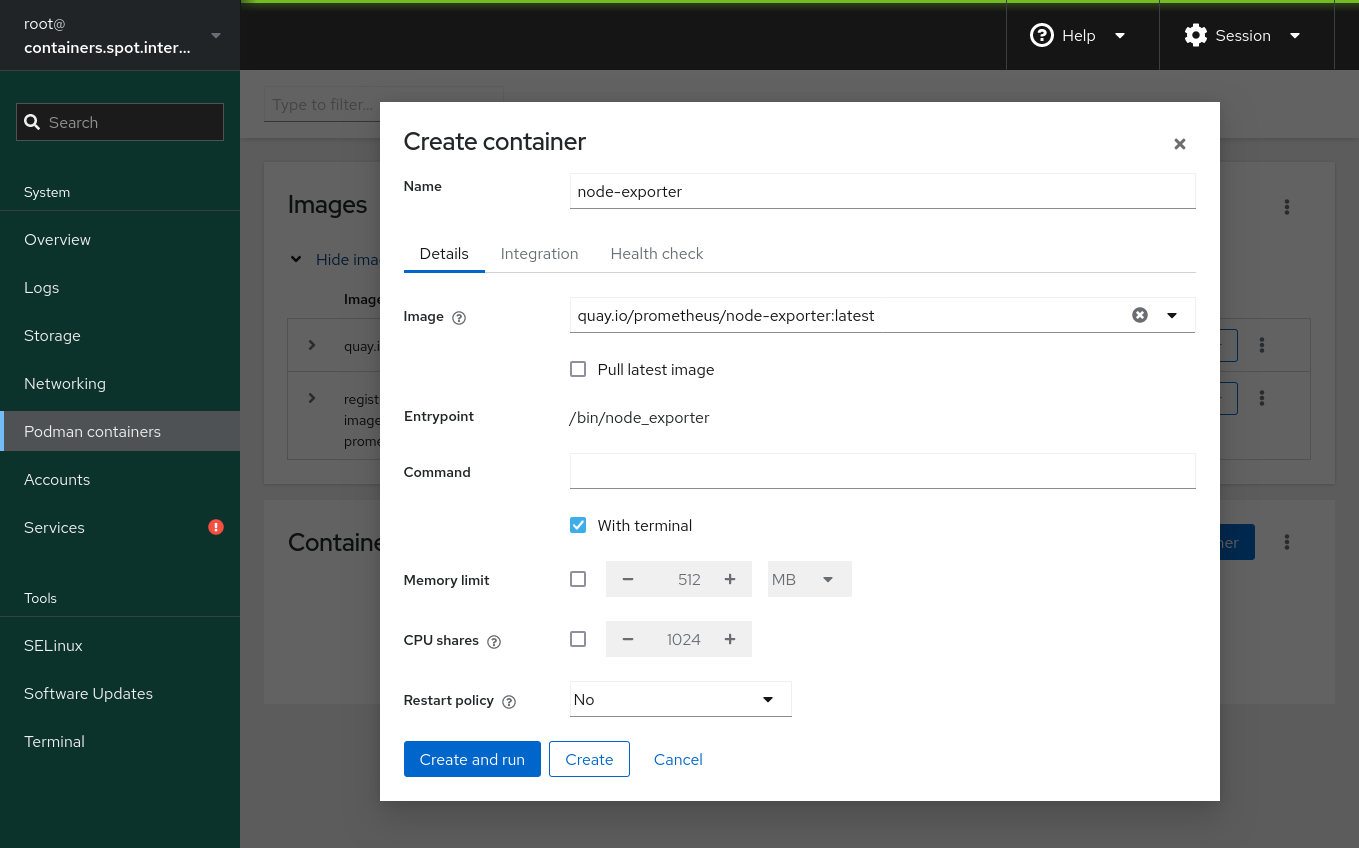
\includegraphics[width=15cm]{figures/cockpit.png}
	\caption{Konténer létrehozása openSUSE Leap Micro-n, a Cockpit webes felületén keresztül.}
	\label{fig:cockpit-container}
\end{figure}

Az openSUSE-projekt kétféle MicroOS-verziót tart karban: a MicroOS-t, mely egy rolling release modellt követ, azaz a rendszer folyamatosan (akár napi szinten) kapja meg a frissítéseket, így több, kisebb verzióugrással tartható karban, míg az openSUSE Leap Micro a \acrlong{sle} Micro kiadási modelljét követi, és a Leap-hez hasonlóan bináris kompatibilitást garantál a két verzió között. A tesztkörnyezethez a stabilitás és kompatibilitás miatt a Leap Micro változatot választottam.




\section{Gépmenedzsment: Salt}


\section{Monitoring}

\section{Továbbfejlesztési lehetőségek}